\chapter{Projekt systemu}
\thispagestyle{chapterBeginStyle}
\label{rozdzial2}

\section{Wymagania}
Celem tej pracy jest stworzenie programu, który przyjmuje opis obliczeń (napisany w prezdefiniowanym języku) dla układu kwantowego. Natępnie tworzy układ kwantowy odpowiadający tym obliczeniom i symuluje jego działanie.
\subsection{Założenia dotyczące opisu wejściowego}
Opis wejściowy (język wejściowy) powinien pozwalać na niżej opisane działania.
\begin{enumerate}
    \item Zefiniowanie zmiennej oraz nadanie jej wartości początkowej (0 lub 1).
    \item Zdefiniowanie dowolnej funkcji boolowskiej na wcześniej zdefiniowanych zmiennych.
    \item Wprowadzenie zmiennej w stan superpozycji, taki, że prawdopodobieństwo otrzymania 0 w wyniku mierzenia wynosi $\frac{1}{2}$.
\end{enumerate}
\subsection{Założenia dotyczące zwracanego wyniku}
Program powinien zwrócić
\begin{enumerate}
    \item Układ kwantowy w postaci stanu początkowego rejestru oraz serii bramek.
    \item Wynik symulacji.
\end{enumerate}
\subsection{Wymagania dodatkowe}
Sposób translacji układu logicznego do kwantowego powinien być taki, by minimalizował liczbę używanych kubitów pomocniczych.
\section{Architektura systemu}
Na rysunku \ref{fig:potok} widać diagram potoku systemu. Program na wejściu przyjmuje opis obliczeń wyspecyfikowany przy użyciu z góry zdefiniowanego języka wejściowego. Opis ten jest parsowany na obiekty rozumiane przez język programowania, przy okazji jest sprawdzana poprawność leksykalna oraz semantyczna zdefiniowanych w opisie wejściowym instrukcji. Wszystkie instrukcje są tłumaczone na akcje związane z układem kwantowym, czyli powiększanie wielkość rejestru kubitów (deklaracja) lub operowanie na rejestrze za pomocą bramek kwantowych. Następnie symulowane jest działanie tak powstałego układu kwantowego. Program zwraca schemat utworzonego układu kwantowego oraz wynik symulacji.
\begin{figure}[H]
    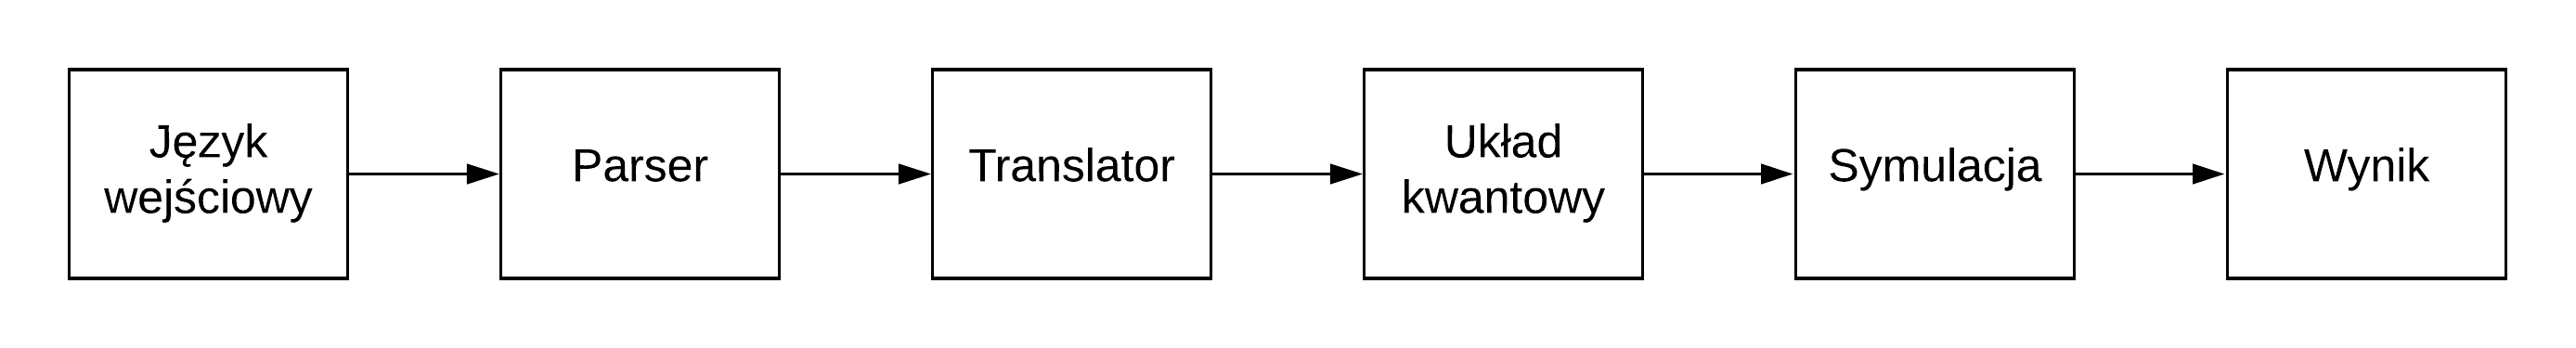
\includegraphics[width=\linewidth]{systemDiag.png}
    \caption{Diagram potoku}
    \label{fig:potok}
\end{figure}
\section{Język wejściowy i parser}
\subsection{Gramatyka}
\begin{tabular}{ l c l } 
    \texttt{\textbf{P}} & $\rightarrow$ & \texttt{\textbf{E} \textbf{P} $|$ \textbf{E}} \\ 
    \texttt{\textbf{E}} & $\rightarrow$ & \texttt{var = \textbf{V} $|$ \textbf{Q}} \\ 
    \texttt{\textbf{V}} & $\rightarrow$ & \texttt{var $|$ const $|$ \textbf{K}} \\ 
    \texttt{\textbf{W}} & $\rightarrow$ & \texttt{\textbf{V} , \textbf{W} $|$ \textbf{V}} \\
    \texttt{\textbf{K}} & $\rightarrow$ & \texttt{and( \textbf{W} ) $|$ not( \textbf{V} ) $|$ or( \textbf{W} ) $|$ xor( \textbf{W} )}\\
    \texttt{\textbf{Q}} & $\rightarrow$ & \texttt{hdm( var ) $|$ swp( var , var ) $|$ tfl( \textbf{L} var \textbf{R} ) $|$ \textbf{F}}\\
    \texttt{\textbf{F}} & $\rightarrow$ & \texttt{frd( : var , var , var ) $|$ frd( var , : var , var ) $|$ frd( var , var , : var )}\\
    \texttt{\textbf{L}} & $\rightarrow$ & \texttt{\textbf{L} : var , $|$ $\epsilon$}\\
    \texttt{\textbf{R}} & $\rightarrow$ & \texttt{, : var \textbf{R} $|$ $\epsilon$}\\
\end{tabular}
\subsection{Analiza leksykalna}
\begin{center}
    \begin{tabular}{|m{4cm}|m{4cm}|p{7cm}|}
        \hline
        Token & Regex & Opis \\
        \hline
        \texttt{var} & \texttt{[a-zA-Z\_]+} & nazwa zmiennej\\
        \texttt{const} & \texttt{0|1} & stała (możliwe wartości początkowe zmiennej)\\
        \texttt{=} & \texttt{=} & operator przypisania\\
        \texttt{,} & \texttt{,} & separator\\
        \texttt{:} & \texttt{:} & wskaźnik kubitu sterującego\\
        \texttt{and(} ( \texttt{not(}, \texttt{or(}, \texttt{xor(} ) & \texttt{and(} ( \texttt{not(}, \texttt{or(}, \texttt{xor(} ) & otwarcie bramki and (not, or, xor)\\
        \texttt{hdm(} ( \texttt{frd(}, \texttt{swp(}, \texttt{tfl(} ) & \texttt{hdm(} ( \texttt{frd(}, \texttt{swp(}, \texttt{tfl(} ) & otwarcie bramki Hadamarda (Fredkina, SWAP, Toffoliego)\\
        \texttt{)} & \texttt{)} & nawias zamykający \\
        \hline
    \end{tabular}
\end{center}
\subsection{Instrukcje i analiza semantyczna}
\subsubsection{Definiowanie zmiennej poprzez przypisanie jej wartości}
\begin{center}
    \textbf{E} $\rightarrow^*$ var = const
\end{center}
Przypisanie wartości zmiennej jest równe jej deklaracji. Raz zadeklarowanej zmiennej nie można przypisać nowej wartości.
\par Na przykład \texttt{a = 0} jest deklaracją zmiennej o nazwie \texttt{a} z wartością równą 0.
\subsubsection{Obliczenie funkcji boolowskiej na wcześniej zadeklarowanych zmiennych.}
\begin{center}
    \textbf{E} $\rightarrow^*$ var = \textbf{K}
\end{center}
Funkcję boolowską definiuje się poprzez bramki logiczne \texttt{and, or, xor, not}. Bramki \texttt{and, or, xor} są uogólnione do dowolnej liczby zmiennych. Instrukcja ta przypisuje wynik funkcji do zmiennej o nazwie $var$ (leksemu odpowiadającemu temu tokenowi). Zmienna o nazwie $var$ nie może być wcześniej zadeklarowana. Instrukcja ta nie zmienia wartości argumentów funkcji \texttt{and, or, xor, not}. 
\par Na przykład instrukcja \texttt{v = and(a,or(c,not(d)))}, gdzie \texttt{a,b,c} to wcześniej zdefiniowane zmienne, przypisze wartość wyrażenia $\texttt{a} \land (\texttt{c} \lor \neg \texttt{d})$ do zmiennej o nazwie \texttt{f}.
\subsubsection{Operowanie na zdefiniowanych zmiennych przy użyciu wybranych bramek kwantowych.}
\begin{center}
    \textbf{E} $\rightarrow^*$ \textbf{Q}
\end{center}
Bramki kwantowe operują na zadeklarownych zmiennych mutując ich stan. Nie zwracają żadnej wartości.
\par Dla bramek wielokubitowych, które przyjmują zmienne sterujące oraz wejściowe, zmienne sterujące oznaczane są poprzez poprzedzający '\texttt{:}'. Na przykład instrukacja \texttt{tfl(:a, b, :c)} oznacza bramkę Toffoliego na zmiennej wejściowej \texttt{b} ze zmiennymi sterującymi \texttt{a}, \texttt{c}.\\
\par Język ten spełnia wcześniej opisane wymagania.
\section{Translator}
Opis zagadnienia translacji został wydzielony do rodziału \ref{rozdzial2a}.
\section{Układ kwantowy z rejestrem}
Przez układ kwantowy z rejestrem rozumiemy tutaj parę $(\q, G)$, gdzie $\q$ to stan wejściowy rejestru kubitów, rozumiany jako wektor, a $G$ to ciąg kolejno nakładanych na rejestr bramek. Każda z bramek, na których użycie pozwala omawiany program należy do jednego z poniższych typów:
\begin{itemize}
    \item[\texttt{hdm}] Bramka Hadamarda
    \item[\texttt{tfl}] Uogólniona bramka Toffoliego
    \item[\texttt{frd}] Bramka Fredkina
    \item[\texttt{swp}] Bramka $SWAP$
\end{itemize}
Poza typem, każda bramka zawiera listę parametów. Dla bramki Hadamarda jest to indeks kubitu, w rejestrze kubitu wejściowego. Bramka Toffoliego jest paramatryzowana, poza indeksem kubitu wejściowego (z ang. \textit{target}), przez listę ideksów kubitów sterujących (z ang. \textit{conrol}). Bramka $SWAP$ jest paramatryzowana parą indeków kubitów wejściowych, a bramka Fredkina parą indeków kubitów wejściowych oraz indeksem kubitu sterującego.
\subsection{Przykład}
Następującemu układowi kwantowemu
\[
    \Qcircuit @C=1.5em @R=1.5em {
        \lstick{\ket{0}} & \targ & \ctrl{2} & \qswap & \qw & \rstick{\ket{o_0}} \qw \\
        \lstick{\ket{0}} & \targ & \qw & \qswap & \gate{H} & \rstick{\ket{o_1}} \qw \\
        \lstick{\ket{0}} & \qw & \targ & \ctrl{-2} &\targ & \rstick{\ket{o_2}} \qw \\
        \lstick{\ket{0}} & \qw & \ctrl{-1} & \gate{H} & \qw & \rstick{\ket{o_3}} \qw
    }
\]
odpowiada specyfikacja $(\q, G)$, gdzie
\[\q = \ket{0000}\]
\begin{center}
    $G$ = [ \texttt{not}(0), \texttt{not}(1), \texttt{tfl}([0,3])(2), \texttt{frd}(2)(0,1), \texttt{hdm}(1), \texttt{not}(2)
\end{center}
a '[]' oznacza uporządkowaną kolekcję elementów.
Porządek wykonywania bramek jest nadany od lewej do prawej. Dla bramek znajdujących się w tej samej kolumnie kolejność wykonywania jest nieistotna.
\section{Symulator}
Ciąg sperametryzowanych bramek przekształcany jest na ciąg macierzy odpowidających tym bramkom, a następnie przeprowadzana jest operacja mnożenia, która kondensuje listę przekształceń do pojedynczej macierzy $M$. W wyniku opracji monożenia macierzy $M$ przez wektor stanu rejestru otrzymywany jest stan końcowy rejestru. Następnie stan ten jest "mierzony", to znaczy zwracany jest losowo, z prawdopodobieństwem wynikającym ze stanu rejestru, jeden z możliwych do zmierzenia stanów. 
\subsection{Generacja macierzy bramek z ich definicji}
Żeby możliwe było mnożenie macierzy bramki przez stanu rejestru macierz ta musi mieć wymiary $2^n \times 2^n$ dla $n$ kubitowego rejestru. Zatem wszystkie bramki operujące na podzbiorze kubitów z rejestru muszą być rozszerzone tak, by operować na całym rejestrze.
\subsubsection{Bramki jednokubitowe}
\label{oneqgate}
Niech $M$ będzie macierzą bramki operujacej na jednym kubicie. Niech $\q$ będzie rejestrem n kubitów.
Weźmy bramkę o macierzy $M$, która operuje na kubicie o indeksie $i < n$ (kubity numerowane od zera).
\par W celu obliczenia wyniku operacji tej bramki na stanie kwantowym $\q$ należałoby pomnożyć macierz $M$ przez stan kubitu z indeksem $i$. Na stanach pozostałych kubitów należy przeprowadzić operację identyczności (której odpowiada macierz identyczności). Operacja łacząca stany kubitów oraz macierze operacji na pojedynczych kubitach to produkt tensorowy oznaczany $\otimes$.
\par Bramka kwantowa $M$ po rozszerzeniu do n kubitów wygląda następująco
\[M_n = Id^i \otimes M \otimes Id^{n-i-1}\]
gdzie przez $Id^j$ dla $j \in \mathbb{N}$ rozumiemy produkt tensorowy $j$ macierzy identyczności o wymiarach $2 \times 2$.
\subsubsection{Bramki wielokubitowe}
\label{multiqg}
Analogicznie można rozszerzać bramki wielokubitowe jeśli operują na sąsiadujących w rejestrze kubitach.
Jeżeli jednak bity sterujące lub bity wejściowe nie sąsiadują to można wykorzystać bramkę $SWAP$ do zamiany kolejności kubitów w rejestrze. Dzięki temu, że każdą permutację można rozbić na złożenie transpozycji, jest to zawsze możliwe do osiągnięcia.
\par Weźmy na przykład układ o rejetrze pięciokubitowym z bramką \texttt{tfl([0,3])(2)}. Układ ten został przestawiony na schemacie poniżej po lewej stronie. Diagram po prawej stronie jest równoważny temu układowi, ale wykorzystuje jedynie operacje na sąsiednich kubitach.
\columnratio{0.45, 0.1, 0.45}
\begin{paracol}{3}
    \vspace*{\fill}
    \[
        \Qcircuit @C=1.5em @R=1.5em {
            \lstick{\ket{q_0}} & \qw & \qw & \ctrl{2} & \qw & \qw & \rstick{\ket{q_0'}} \qw \\
            \lstick{\ket{q_1}} & \qw & \qw & \qw & \qw & \qw & \rstick{\ket{q_1'}} \qw \\
            \lstick{\ket{q_2}} & \qw & \qw &\targ & \qw & \qw & \rstick{\ket{q_2'}} \qw \\
            \lstick{\ket{q_3}} & \qw & \qw & \ctrl{-1} & \qw& \qw & \rstick{\ket{q_3'}} \qw \\
            \lstick{\ket{q_4}} & \qw & \qw & \qw & \qw & \qw & \rstick{\ket{q_4'}} \qw
        }
    \]
    \vspace*{\fill}
    \switchcolumn
    \vspace*{\fill}
    \centering
    =
    \vspace*{\fill}
    \switchcolumn
    \vspace*{\fill}
    \[
        \Qcircuit @C=1.5em @R=1.5em {
            \lstick{\ket{q_0}} & \qswap & \qw & \qw & \qw & \qswap & \rstick{\ket{q_0'}} \qw \\
            \lstick{\ket{q_1}} & \qswap \qwx & \qw & \ctrl{1} & \qw & \qswap \qwx & \rstick{\ket{q_1'}} \qw \\
            \lstick{\ket{q_2}} & \qw & \qswap &\ctrl{1} & \qswap & \qw & \rstick{\ket{q_2'}} \qw \\
            \lstick{\ket{q_3}} & \qw & \qswap \qwx & \targ & \qswap \qwx & \qw & \rstick{\ket{q_3'}} \qw \\
            \lstick{\ket{q_4}} & \qw & \qw & \qw & \qw & \qw & \rstick{\ket{q_4'}} \qw
        }
    \]  
    \vspace*{\fill}
\end{paracol}
Zatem można rozpisać $\texttt{tfl([0,3])(2)} = \texttt{swp(0,1)} * \texttt{swp(2,3)} * \texttt{tfl([1,2])(3)} * \texttt{swp(0,1)} * \texttt{swp(2,3)}$. Gdy każda z wykorzystwanych bramek zostanie rozszerzona, tak by operowała na pięciu kubitach, zgodnie ze strategią opisaną z tym rozdziale, to zostanie wygenerowana macierz wykonująca operację \texttt{tfl([0,3])(2)} na rejestrze pieciokubitowym.
\subsubsection{Uogólniona bramka Toffoliego}
Uogólniona bramka Toffoliego wykonuje operację negacji na bicie wejściowym, gdy wszystkie bity strerujące są jedynkami.
\par Opisana w niniejszym rozdziale bramka \texttt{tfl([0,3])(2)} operująca na pięciokubitowym rejestrze mapuje czyste stany kwantowe następująco
\[10010  \rightarrow 10110\;\text{ i }\;10110  \rightarrow 10010\] %18 - 22
\[11010  \rightarrow 11110\;\text{ i }\;11010  \rightarrow 11110\] %26 - 30
\[10011  \rightarrow 10111\;\text{ i }\;10011  \rightarrow 10111\] %19 -23
\[11011  \rightarrow 11111\;\text{ i }\;11011  \rightarrow 11111\] %27 - 31
w pozostałych przypadkach dokonuje mapowania identycznościowego.
\par Bramka Toffoliego jest macierzą permutacji, która w każdym wierszu oraz kolumnie ma dokładnie jedną jedynkę oraz $n-1$ zer. Dla mapowania
\[10010  \rightarrow 10110\]
jedynka powinna się znaleźć w 19 kolumnie, 23 wierszu, ponieważ 
\[10010_{(2)} = 18\]
\[10110_{(2)} = 22\]
gdzie numaracja zaczyna się od zera.\vspace{4mm}\\
\begin{pseudokod}[H]
    \SetArgSty{normalfont}
    \KwIn{Liczba kubitów w rejestrze $n$, zbiór indeksów bitów sterujących $C$, indeks bitu wejściowego $i$}
    \KwOut{Macierz bramki Toffoliego M}
    $M \leftarrow$ macierz wymiarów $2^n \times 2^n$ wypełniona 0\;
    \For{$j \leftarrow 0$ \KwTo $2^n$}{
        $isId \leftarrow$ \texttt{false}\;
        \ForEach{$c \in C$}{
            \tcc{bity w zapisie biranym numerujemy od najmiej znaczącego, indeksem 0}
            \If{$j$ ma 0 na ($n-c-1$)-tym bicie w zapisie binarnym}{
                $isId \leftarrow$ \texttt{true} \;
            }
        }
        \If{$isId$}{
            \tcc{przypadek gdy, wszystkie kubity sterujące są jedynkami}
                wstaw 1 do macierzy M na miejscu ($j$, $j$ zanegowane na ($n-i$)-tym bicie) \tcp*{(kolumna, wiersz)}
        }
        \Else {
                wstaw 1 do macierzy M na miejscu ($j$, $j$) \;
        }
    }
    \caption{Generacja macierzy bramki Toffoliego z defninicji bramki}\label{alg:toffoliGateGen}
\end{pseudokod}
\section{Wyjście}
Program zwraca schemat układu kwantowego, który został stworzony w wyniku działania translatora. Układ ten odpowiada obliczeniom zdefiniowanym w opisie wejściowym.
\par Poza układem program zwraca wynik obliczeń, czyli końcowy, zmierzony, stan rejestru kwantowego po symulacji działania układu kwantowego. Dodatkowo zwaraca informację o prawdopodobienstwie otrzymania stanu $\ket{1}$ dla każdego z kubitów w rejestrze.